\documentclass[mathserif]{beamer}
\usepackage{natbib}
\usepackage{bibentry}
\begin{document}
\nobibliography*
\title{Comparing Adaptive Filtering Techniques \\ ENCE689E --- Reading Assignment}
\author{David Prentiss \\ University of Maryland College Park}
\subtitle{With a summary of \\ \bibentry{crow2008comparison}}

\frame{\titlepage}

\begin{frame}
  \frametitle{Crow and Reichle (2008)}
  \tableofcontents
\end{frame}

\section{Land Surface Modeling}

\begin{frame}
  \frametitle{Crow and Reichle (2008)}
  \tableofcontents[currentsection]
\end{frame}

\begin{frame}
  \frametitle{\insertsection}
  \begin{itemize}
    \item Water and Energy Balance Surface Vegetation Atmosphere Transfer (WEB--SVAT)
    \item Point-based, two-state, mass balance (by volume)
    \item Surface zone (5 cm) moisture flux, $\theta_{sz}$
      \begin{equation}
        \frac{d\theta_{sz}}{dt}=\frac{B_1}{d_{sz}}\left(P_g - E_S\right)-\frac{B_2}{\tau}\left(\theta_{sz}-\theta_{eq}\right)
      \end{equation}
    \item Root zone (50 cm), $\theta_{rz}$
      \begin{equation}
        \frac{d\theta_{rz}}{dt}=\frac{1}{d_{rz}}\left(P_g - T - E_S - D\right)
      \end{equation}
    \item Linear or non-linear?
  \end{itemize}
\end{frame}

\section{EnKFs and Adaptive Filters}

\begin{frame}
  \frametitle{Crow and Reichle (2008)}
  \tableofcontents[currentsection]
\end{frame}

\begin{frame}
  \frametitle{\insertsection}
  \begin{itemize}
    \item The measurement error covariance $\mathbf{R}$ reduces to scalar $R$, since $H = (1, 0)$
    \item Model error covariance matrix $\mathbf{Q}$ is assumed to capture all model error (forcing and parameters)
    \item Correlation coefficient $\rho$ known
    \item Ratio of state standard deviations $\alpha$ known
      \begin{equation}
        \mathbf{Q}=\begin{pmatrix}
          Q & \alpha Q \rho \\
          \alpha Q \rho & \alpha^2 Q
        \end{pmatrix}
      \end{equation}
      where
      \begin{equation}
        \sqrt{Q} = \alpha\sigma_{q_1} = \sigma_{q_2}
      \end{equation}
  \end{itemize}
\end{frame}

\section{Synthetic Twin Experiment}

\begin{frame}
  \frametitle{Crow and Reichle (2008)}
  \tableofcontents[currentsection]
\end{frame}

\begin{frame}
  \frametitle{\insertsection}
  \begin{itemize}
    \item Truth: $\alpha = 0.30,\ \rho= 0.70$, and $\sqrt{Q_{true}} = 0.05$ vol/vol
    \item 25-member EnKF
    \item "Stratified grid of guesses" for the initial conditions ($\sqrt{Q_0}$ and $\sqrt{R_0}$)
    \item Daily, synthetic soil moisture observations for 3000 days
    \item Sampling period of 50 days where applicable
    \item Filters compared on their ability to correct initial conditions and converge on the true variances
  \end{itemize}
\end{frame}

\section{Comparison of Four Adaptive Filters}

\begin{frame}
  \frametitle{Crow and Reichle (2008)}
  \tableofcontents[currentsection]
\end{frame}

\begin{frame}
  \frametitle{\insertsection}
  \begin{itemize}
    \item Filter diagnostic $\tilde{v}_t$
    \begin{equation} \tilde{v}_t = E \left[ y_{t,i}-Hx_{t,i-} \right]/(H\mathbf{P_t}H^T+R)^{1/2}\end{equation}
    \item Zero Mean
    \item Serially uncorrelated
    \item Temporal variance of one
  \end{itemize}
\end{frame}

\begin{frame}
  \begin{center}
  \frametitle{\insertsection}
  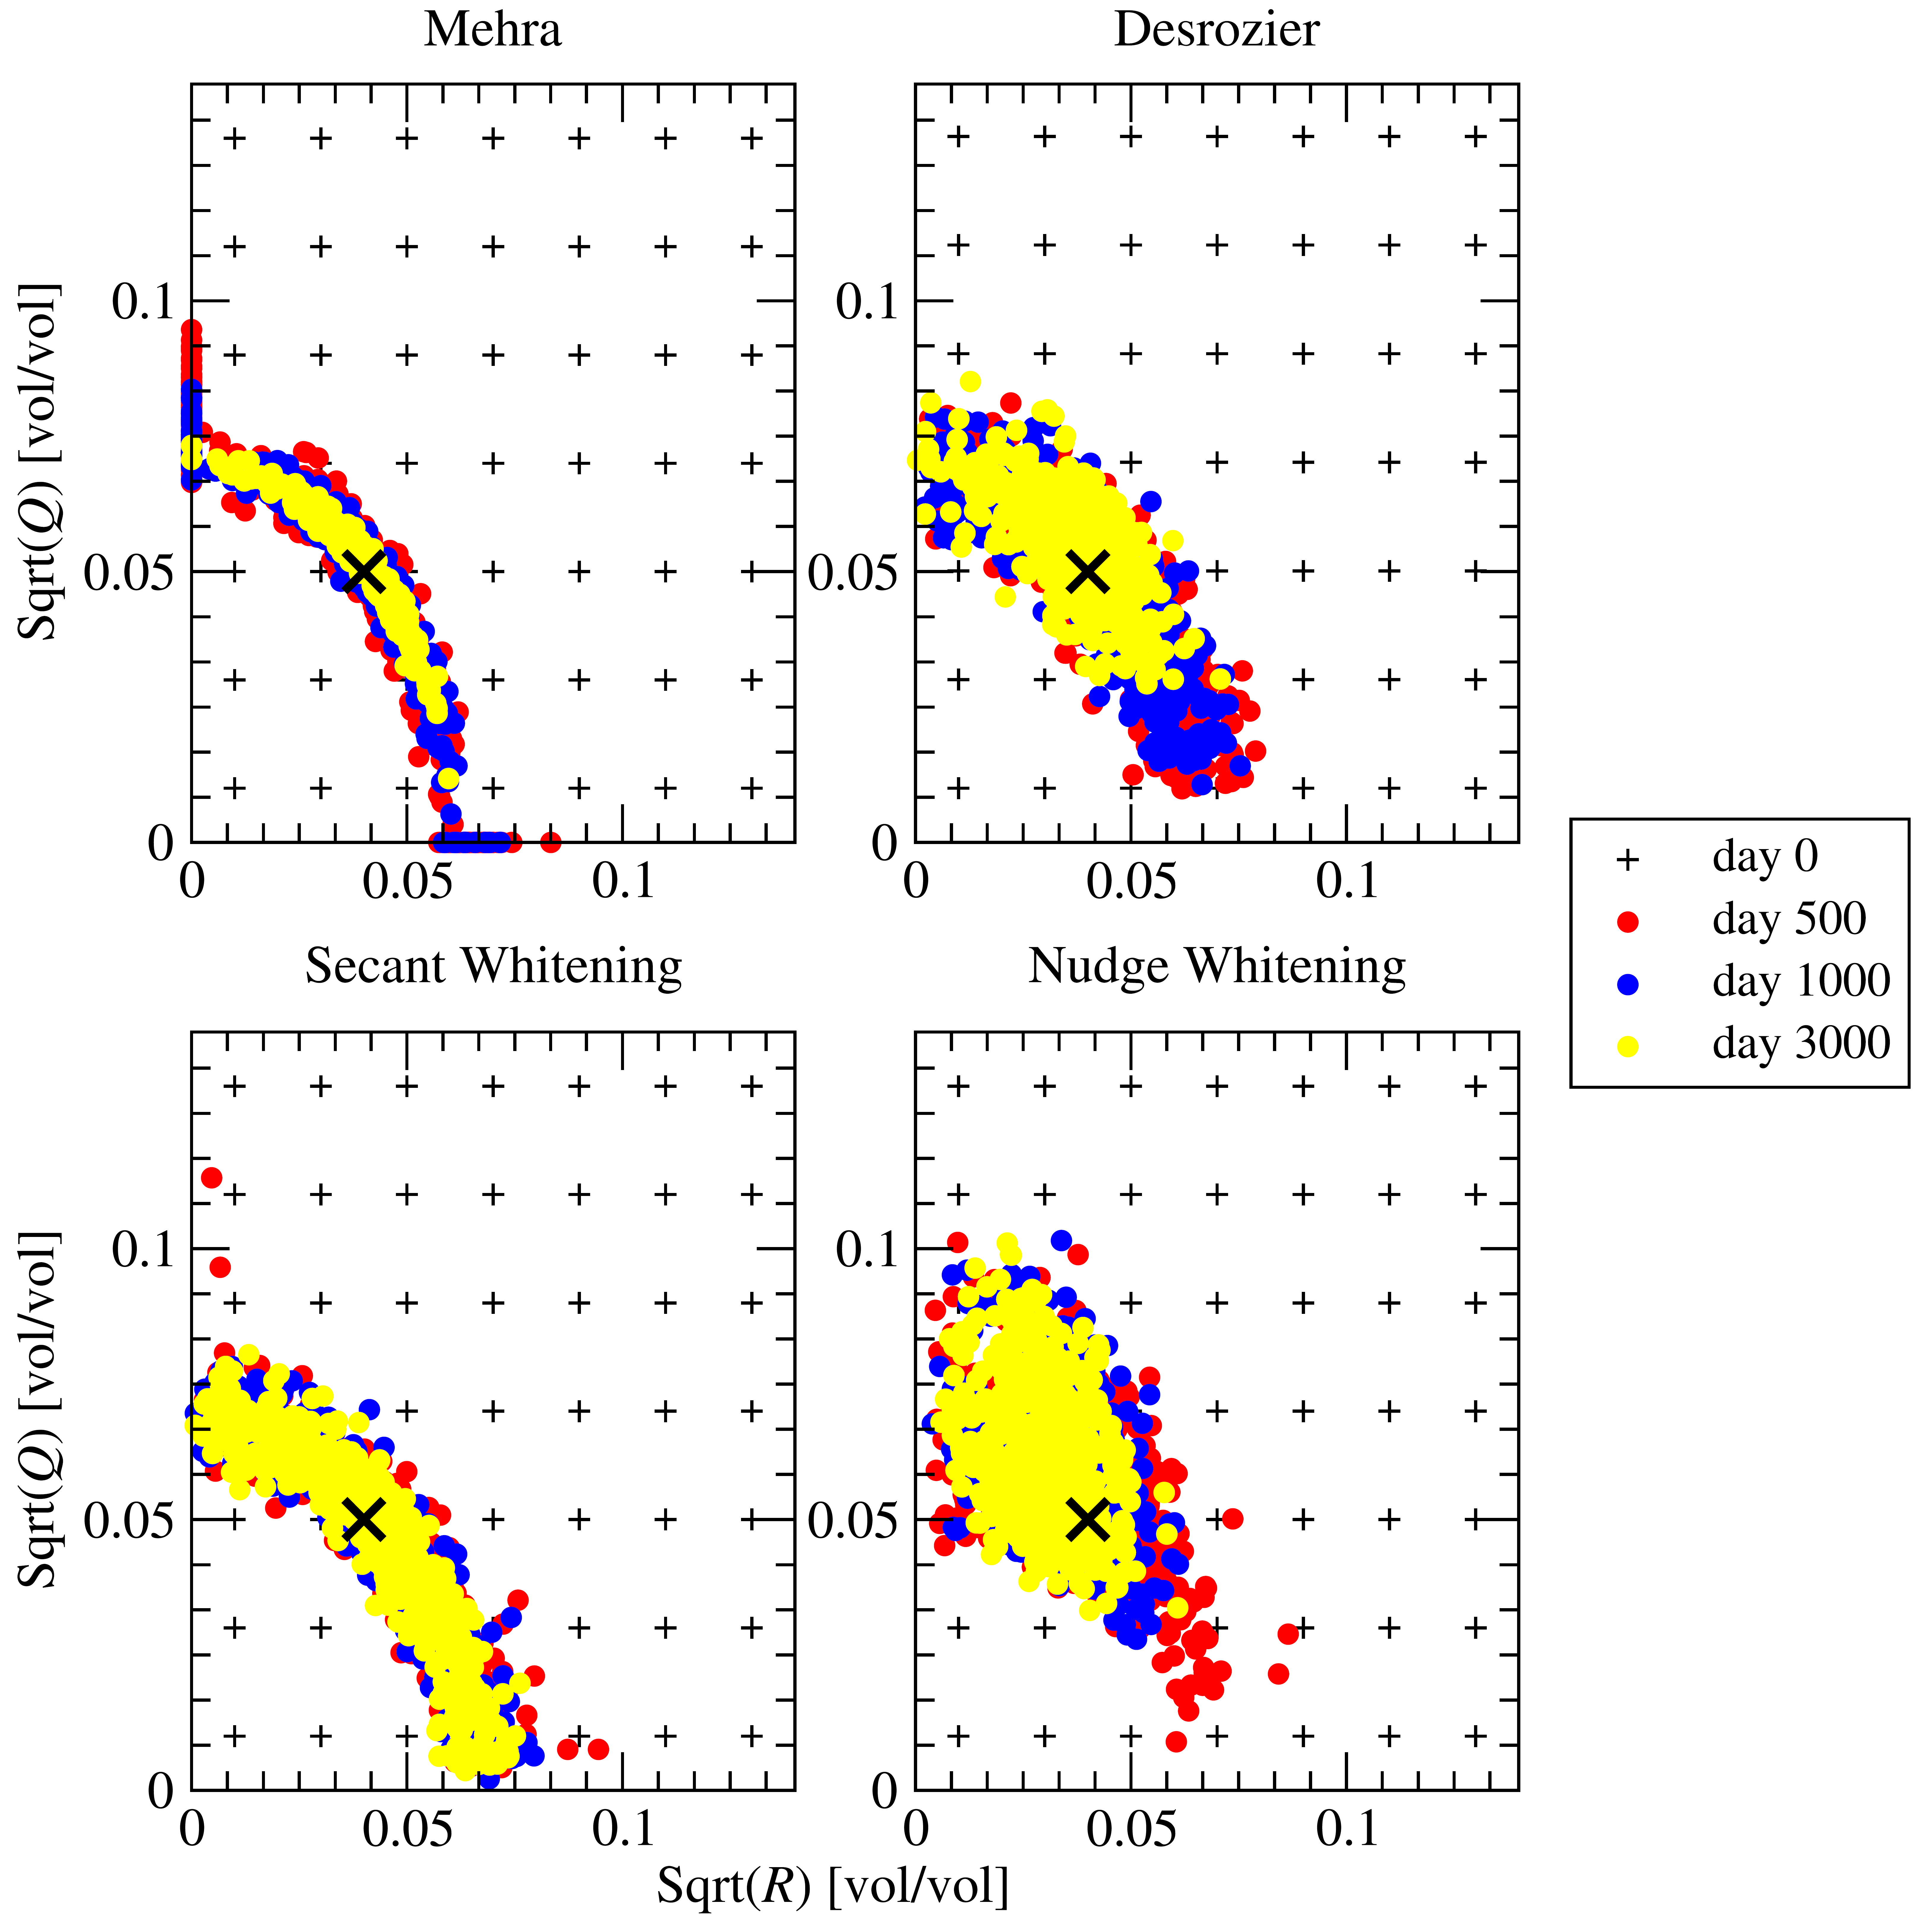
\includegraphics[width=0.8\textwidth]{days}
  \end{center}
\end{frame}

\begin{frame}
  \frametitle{Crow and Reichle (2008)}
\begin{centering}
  Thank you.
\end{centering}
\end{frame}

\bibliographystyle{plainnat}
\bibliography{reading}
\end{document}
